%--------------------------------------------------
\subsection{Prototipo 2: Monitor geográfico de beacons}

%--------------------------------------------------
\subsubsection{Análisis}

Dentro de este prototipo se satisface el requerimiento funcional \hyperlink{RFPA}{Monitorear Beacons y tiendas}, definido previamente en el capítulo del ``Bosquejo general de la aplicación''  con el título de ``Requerimientos funcionales del Panel de Administración''. \\ \par

\FloatBarrier

\title{\textbf{Diagrama de casos de uso \\}}
La figura \ref{casosdeusoPA} muestra todos los casos de uso del Panel de Administración que serán realizados a lo largo de los diferentes prototipos pertenecientes al Panel de Administración.
\FloatBarrier
\begin{figure}[htbp!]
		\centering
			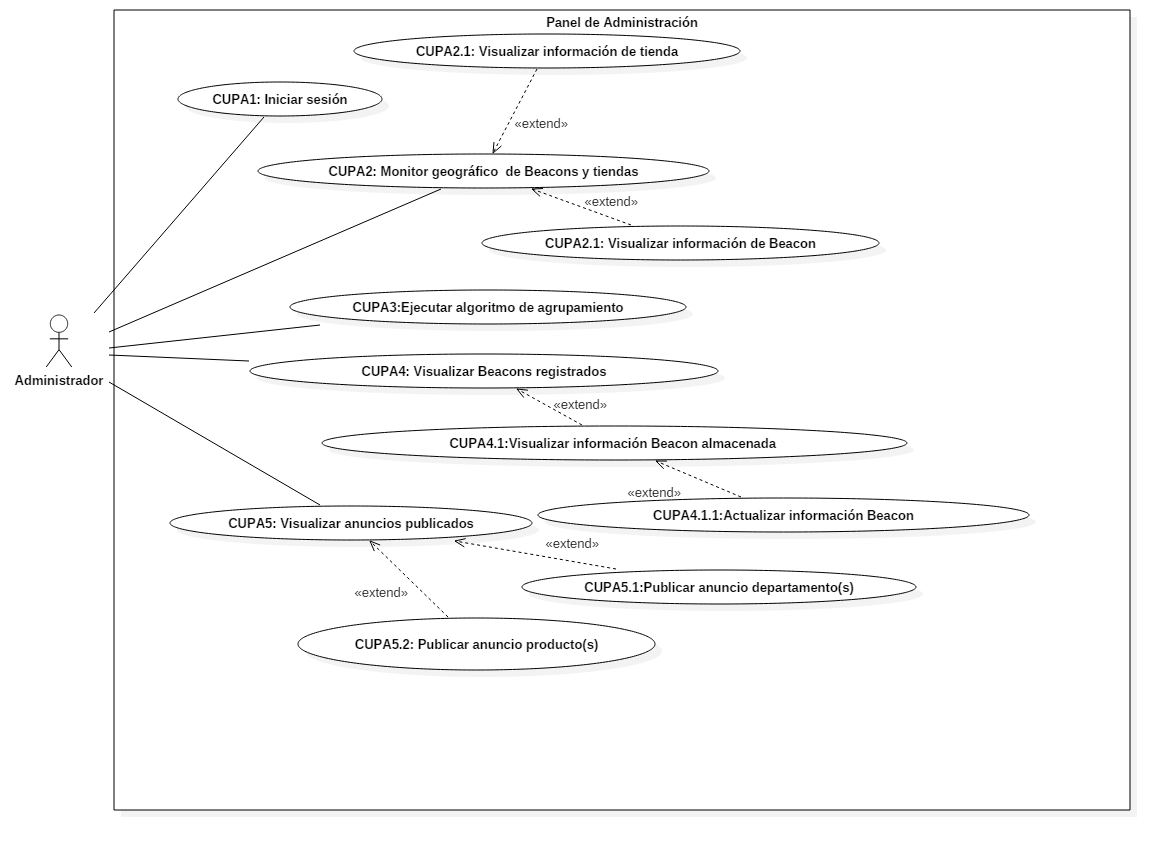
\includegraphics[width=1.1 \textwidth]{imagenes/CU/middleware}
		\caption{Casos de uso PA.}
		\label{casosdeusoPA}
\end{figure}
\FloatBarrier

%--------------------------------------------------
\subsubsection{Diseño}
\title{\textbf{Diagramas de secuencia} \\}
El diagrama de secuencia que satisface el requerimiento dentro de este prototipo se puede ver en la figura \ref{DS:MonitorGeografico}. Para una mejor visualización la figura se repartió en dos secciones que se encuentran en \ref{DS:MonitorGeografico1} y \ref{DS:MonitorGeografico2}. \\
\title{\textbf{Monitor Geográfico de Beacons y tiendas}}

\FloatBarrier
\begin{figure}[htbp!]
		\centering
			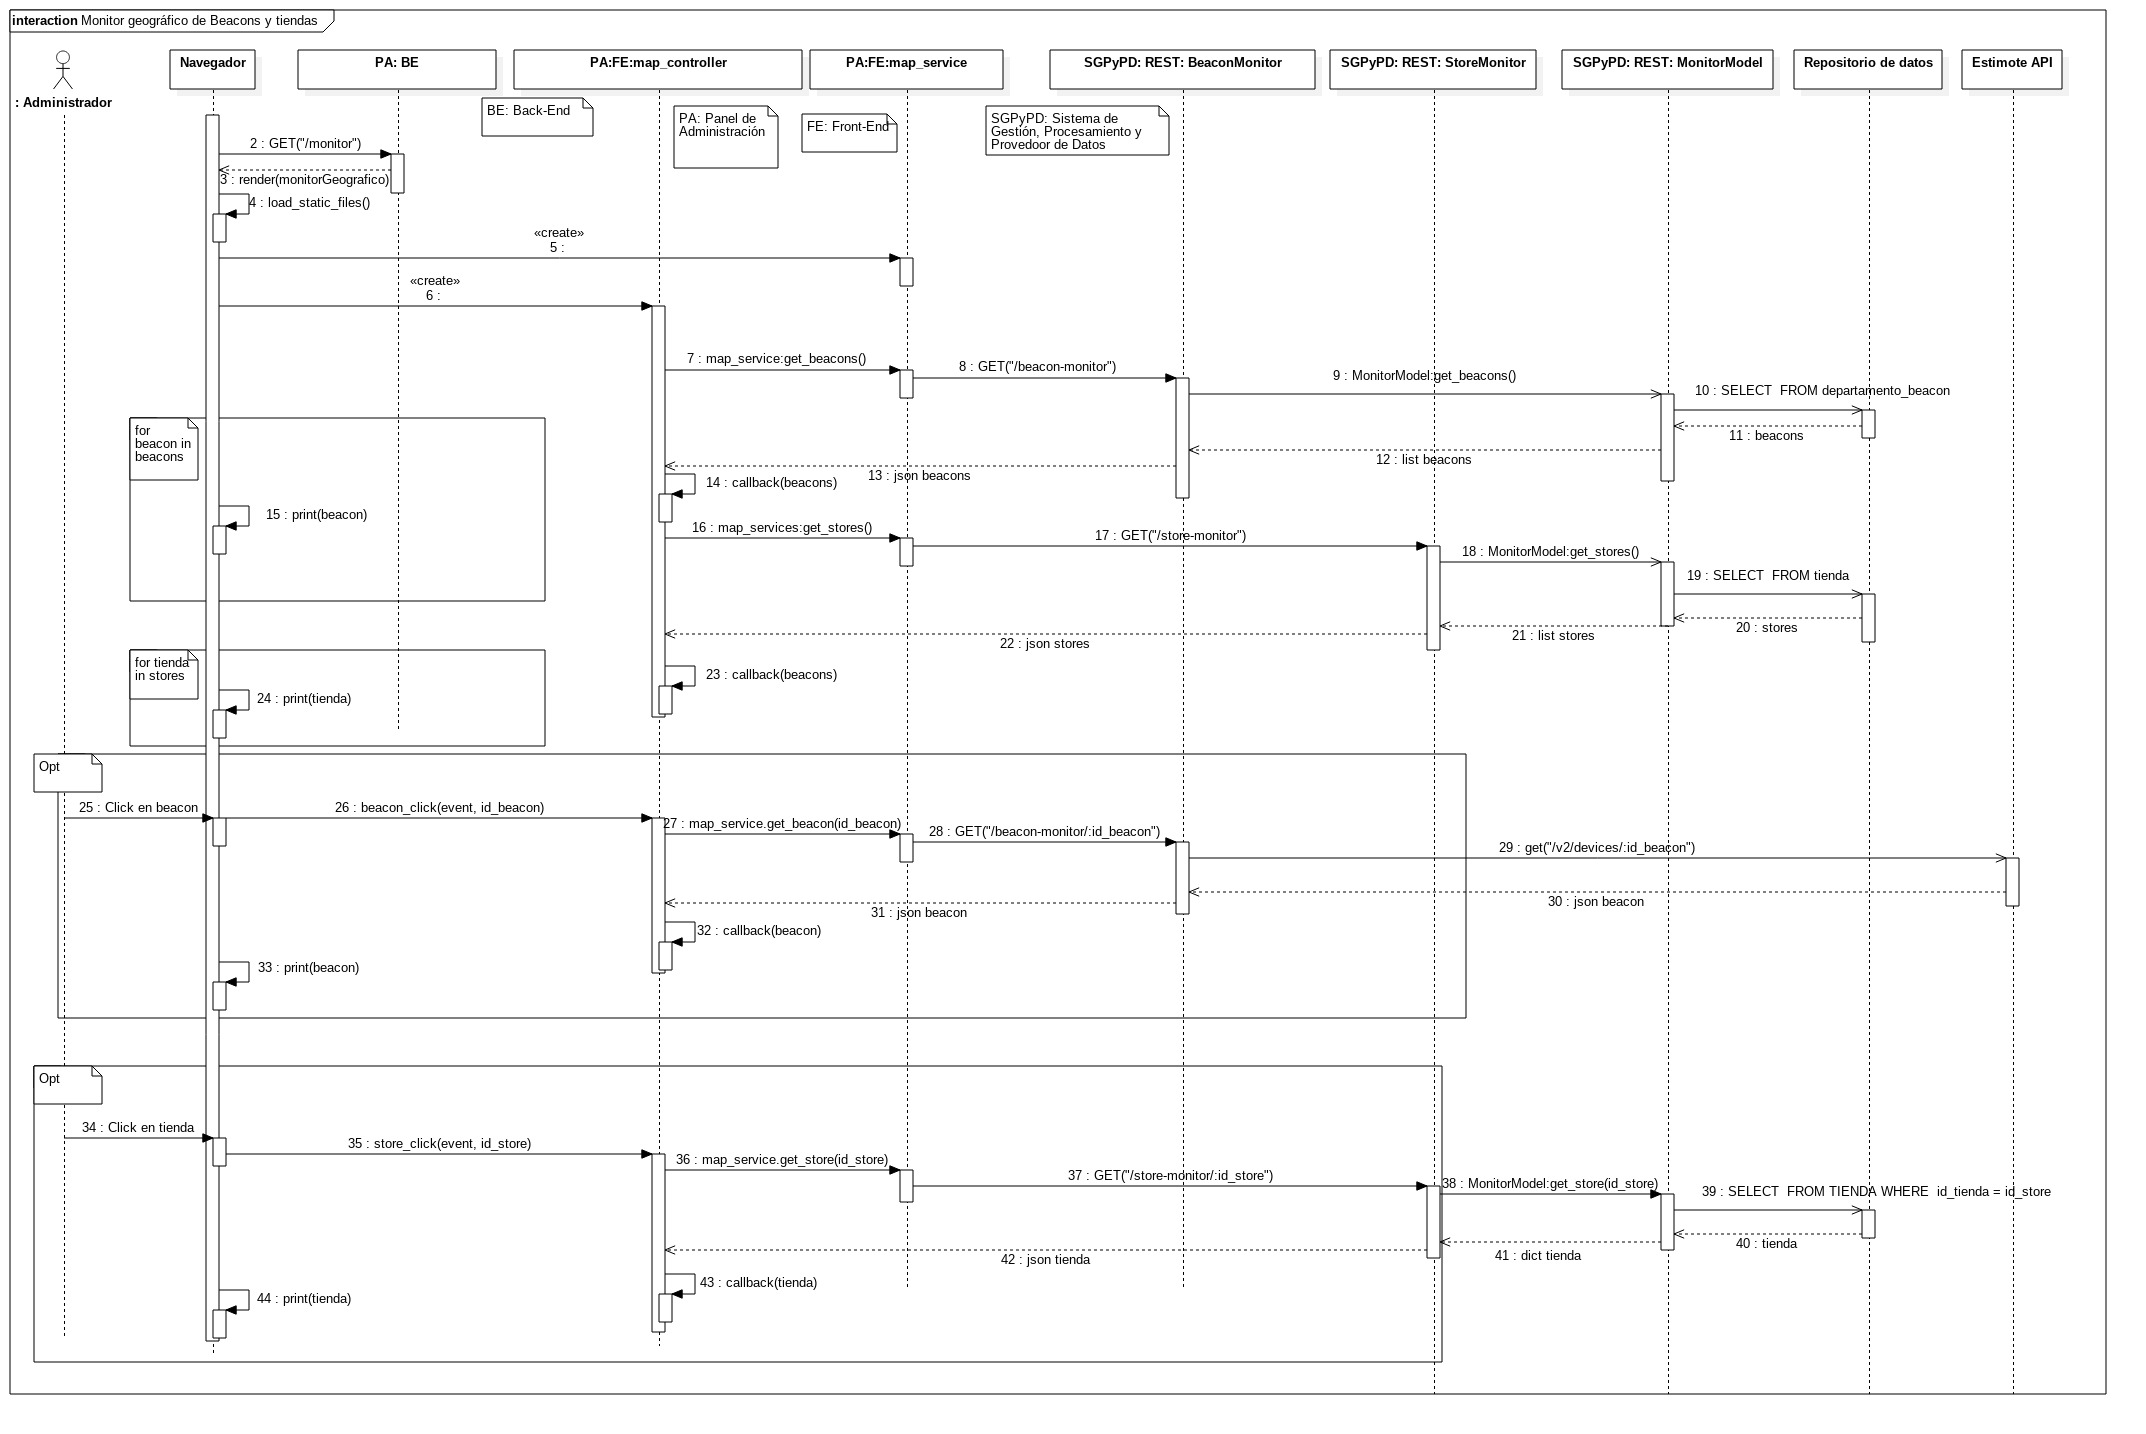
\includegraphics[width=1 \textwidth]{imagenes/DSRuben/MonitorGeografico}
		\caption{Diagrama de secuencia del monitor geográfico (Visualización completa).}
		\label{DS:MonitorGeografico}
\end{figure}
\FloatBarrier

\FloatBarrier
\begin{figure}[htbp!]
		\centering
			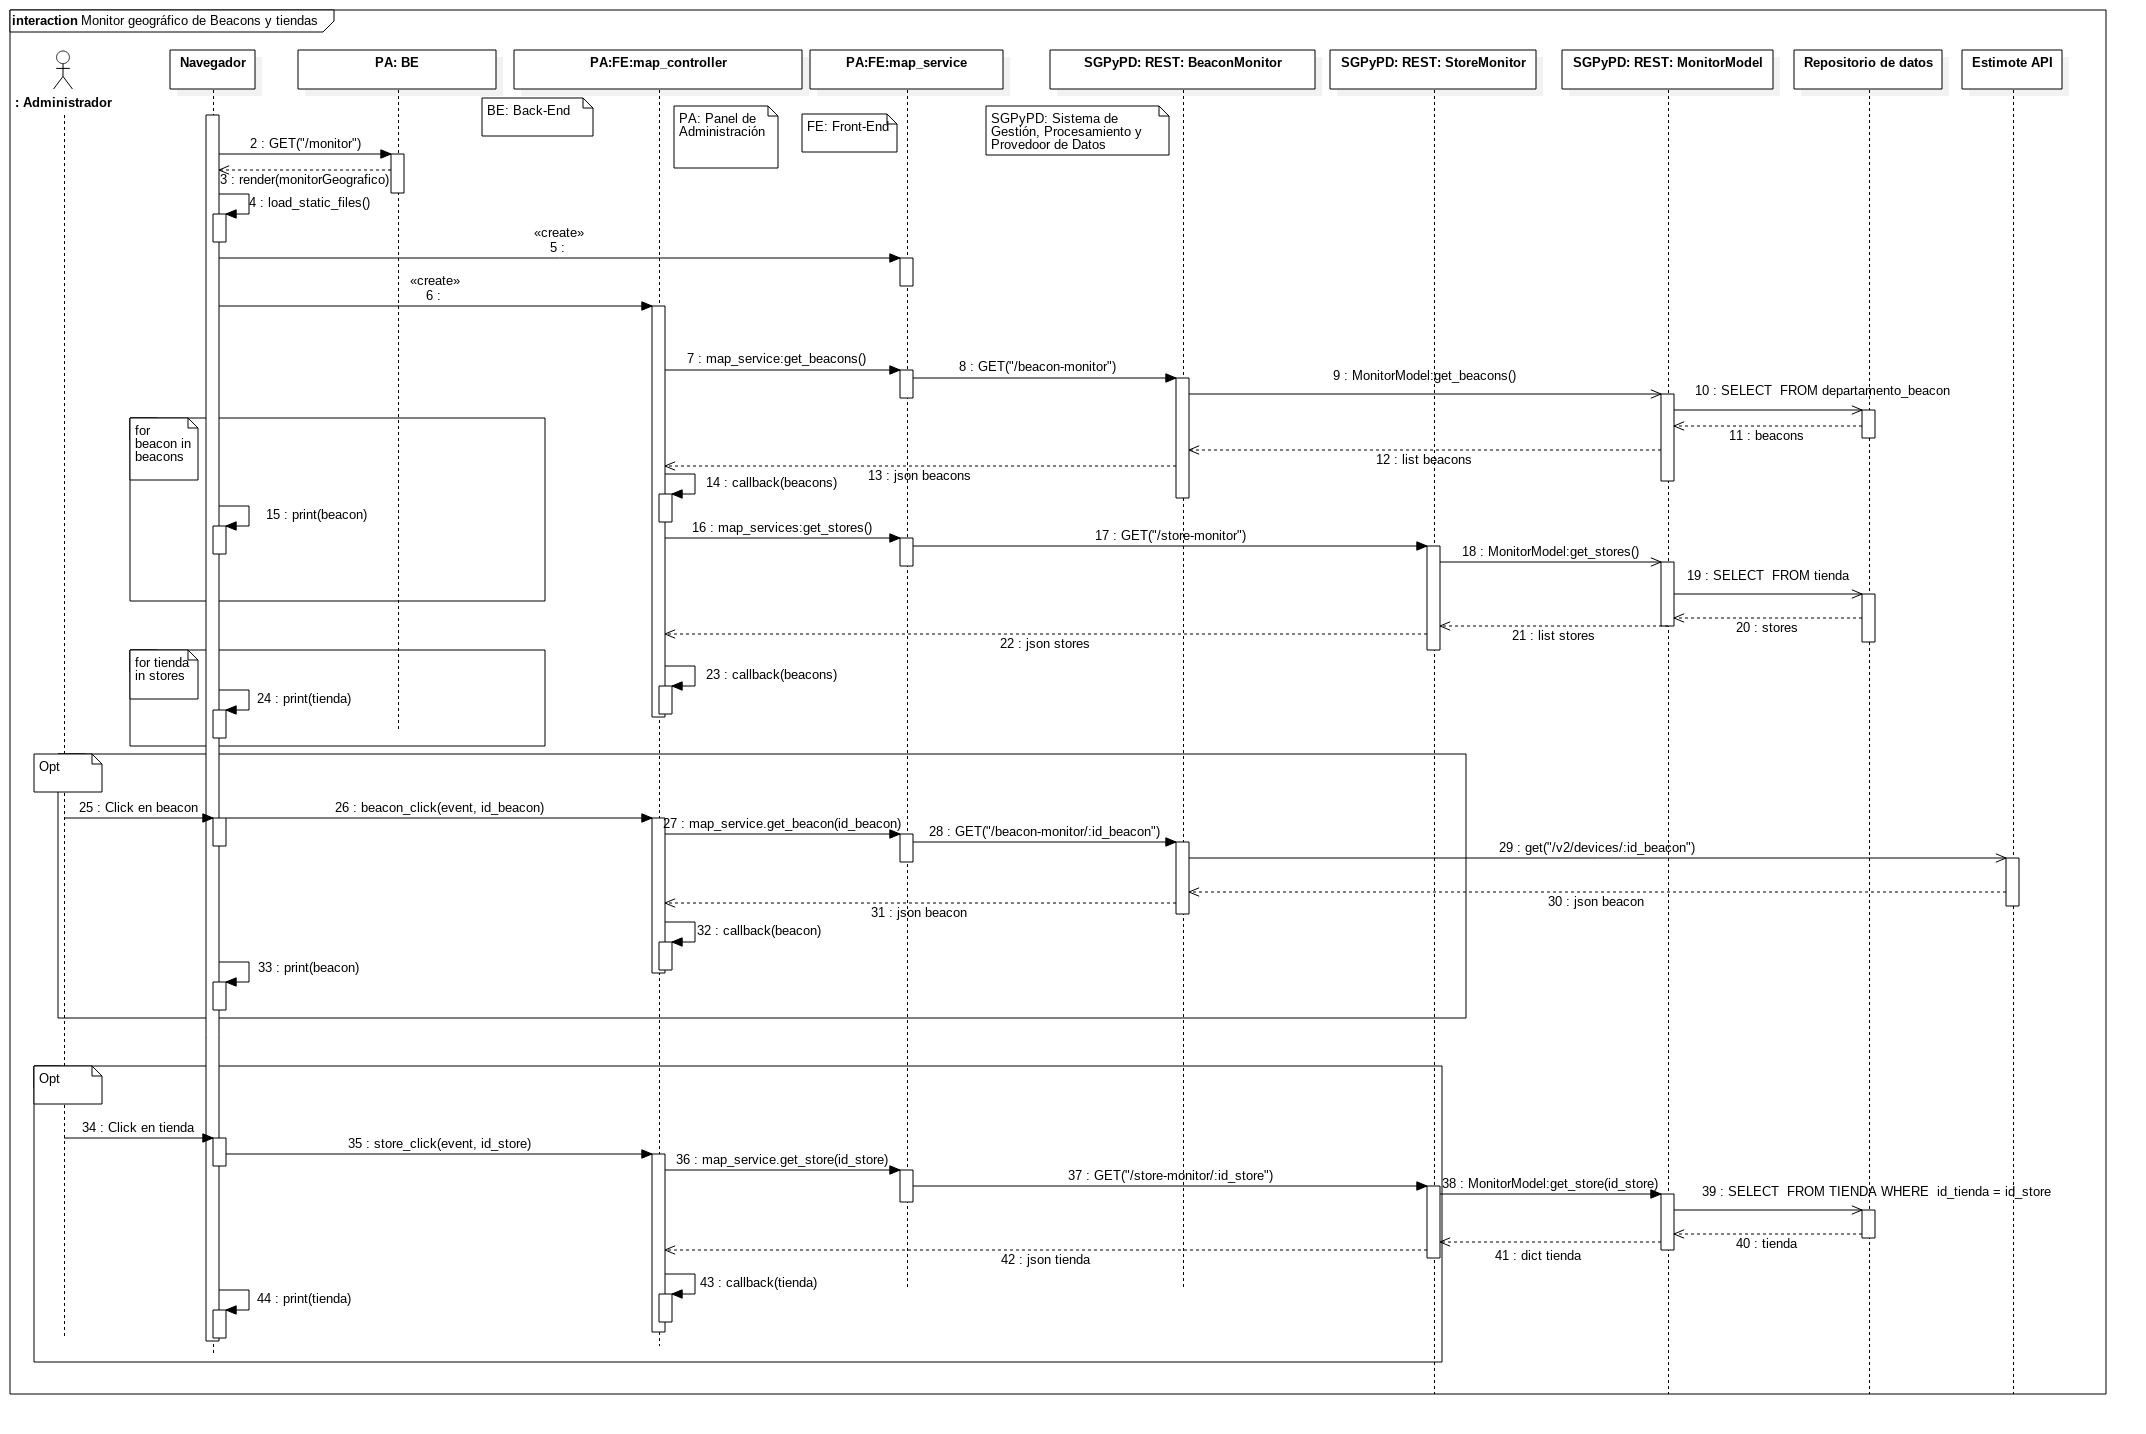
\includegraphics[width=1 \textwidth]{imagenes/DSRuben/MonitorGeografico_1}
		\caption{Diagrama de secuencia del monitor geográfico (Parte 1).}
		\label{DS:MonitorGeografico1}
\end{figure}
\FloatBarrier

\FloatBarrier
\begin{figure}[htbp!]
		\centering
			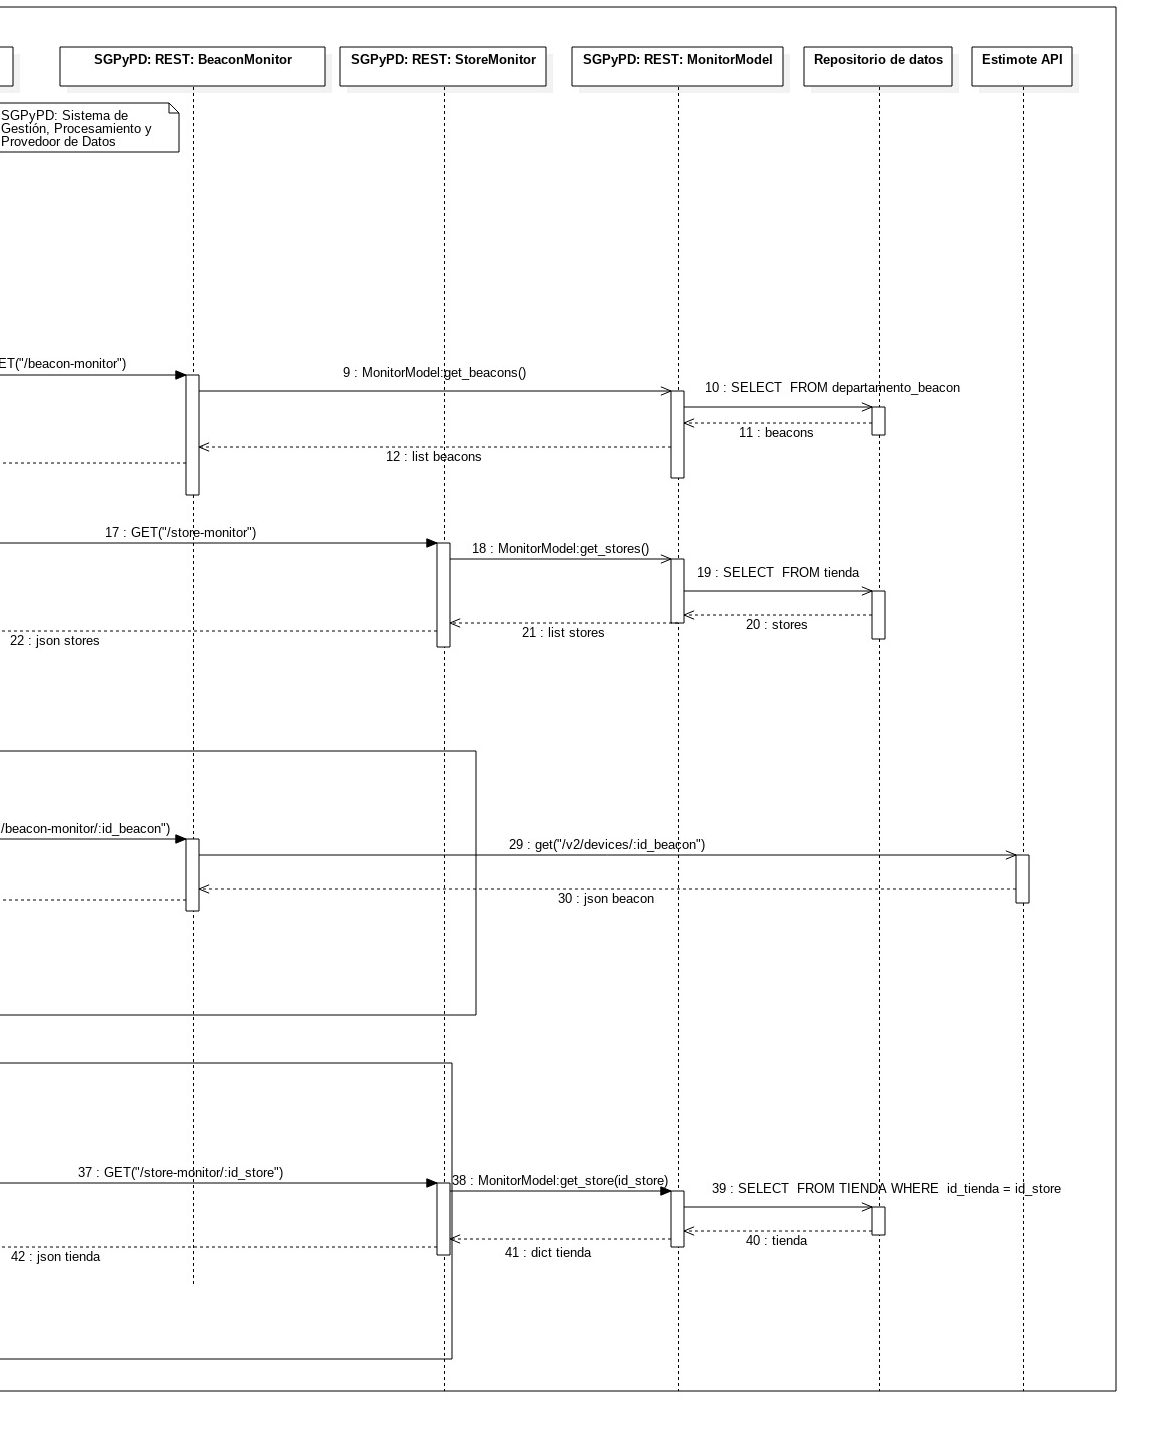
\includegraphics[width=1 \textwidth]{imagenes/DSRuben/MonitorGeografico_2}
		\caption{Diagrama de secuencia del monitor geográfico (Parte 2).}
		\label{DS:MonitorGeografico2}
\end{figure}
\FloatBarrier


\newpage
\title{\textbf{Diseño de interfaz de usuario \\}}
En la imagen \ref{diseniomonitorGeografico} se muestra el resultado de este prototipo.
\FloatBarrier
\begin{figure}[htbp!]
		\centering
			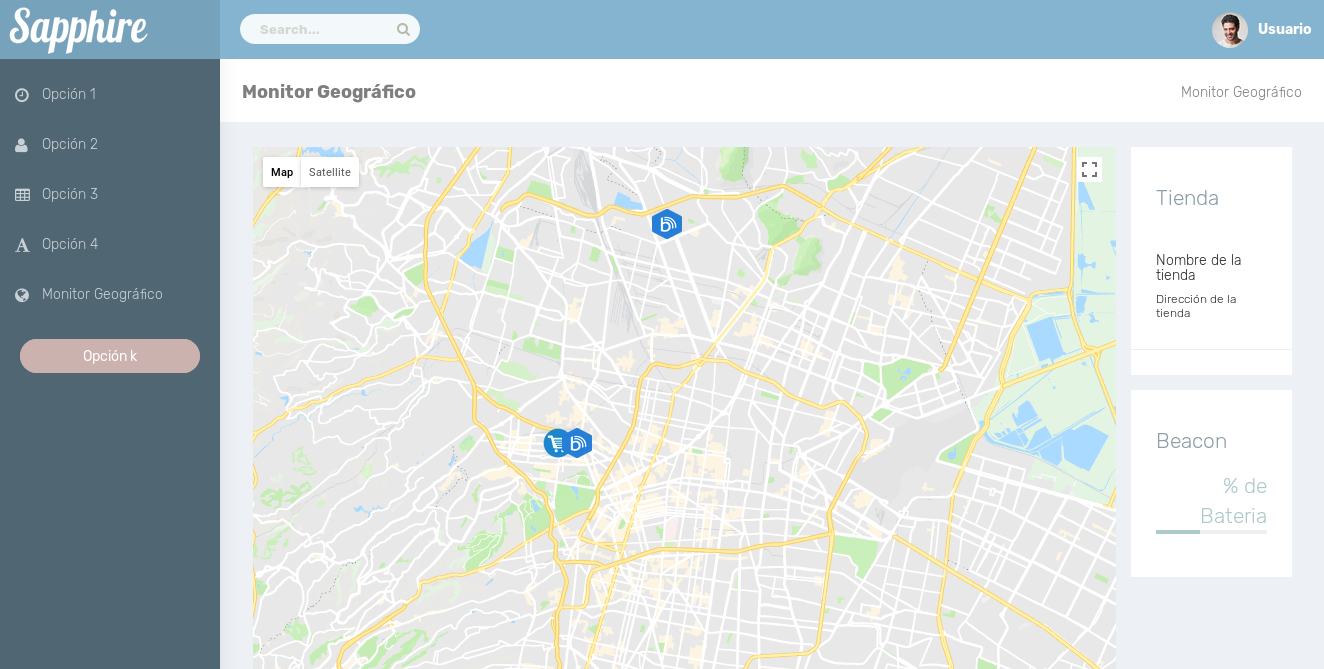
\includegraphics[width=1 \textwidth]{imagenes/UI/middlewareMonitorGeografico}
		\caption{Diseño monitor geográfico.}
		\label{diseniomonitorGeografico}
\end{figure}
\FloatBarrier

La Figura \ref{PA:3} muestra como se ve la interfaz de usuario del Panel de Administración para el monitor de Beacons y tiendas desde una computadora.

\FloatBarrier
\begin{figure}[htbp!]
		\centering
			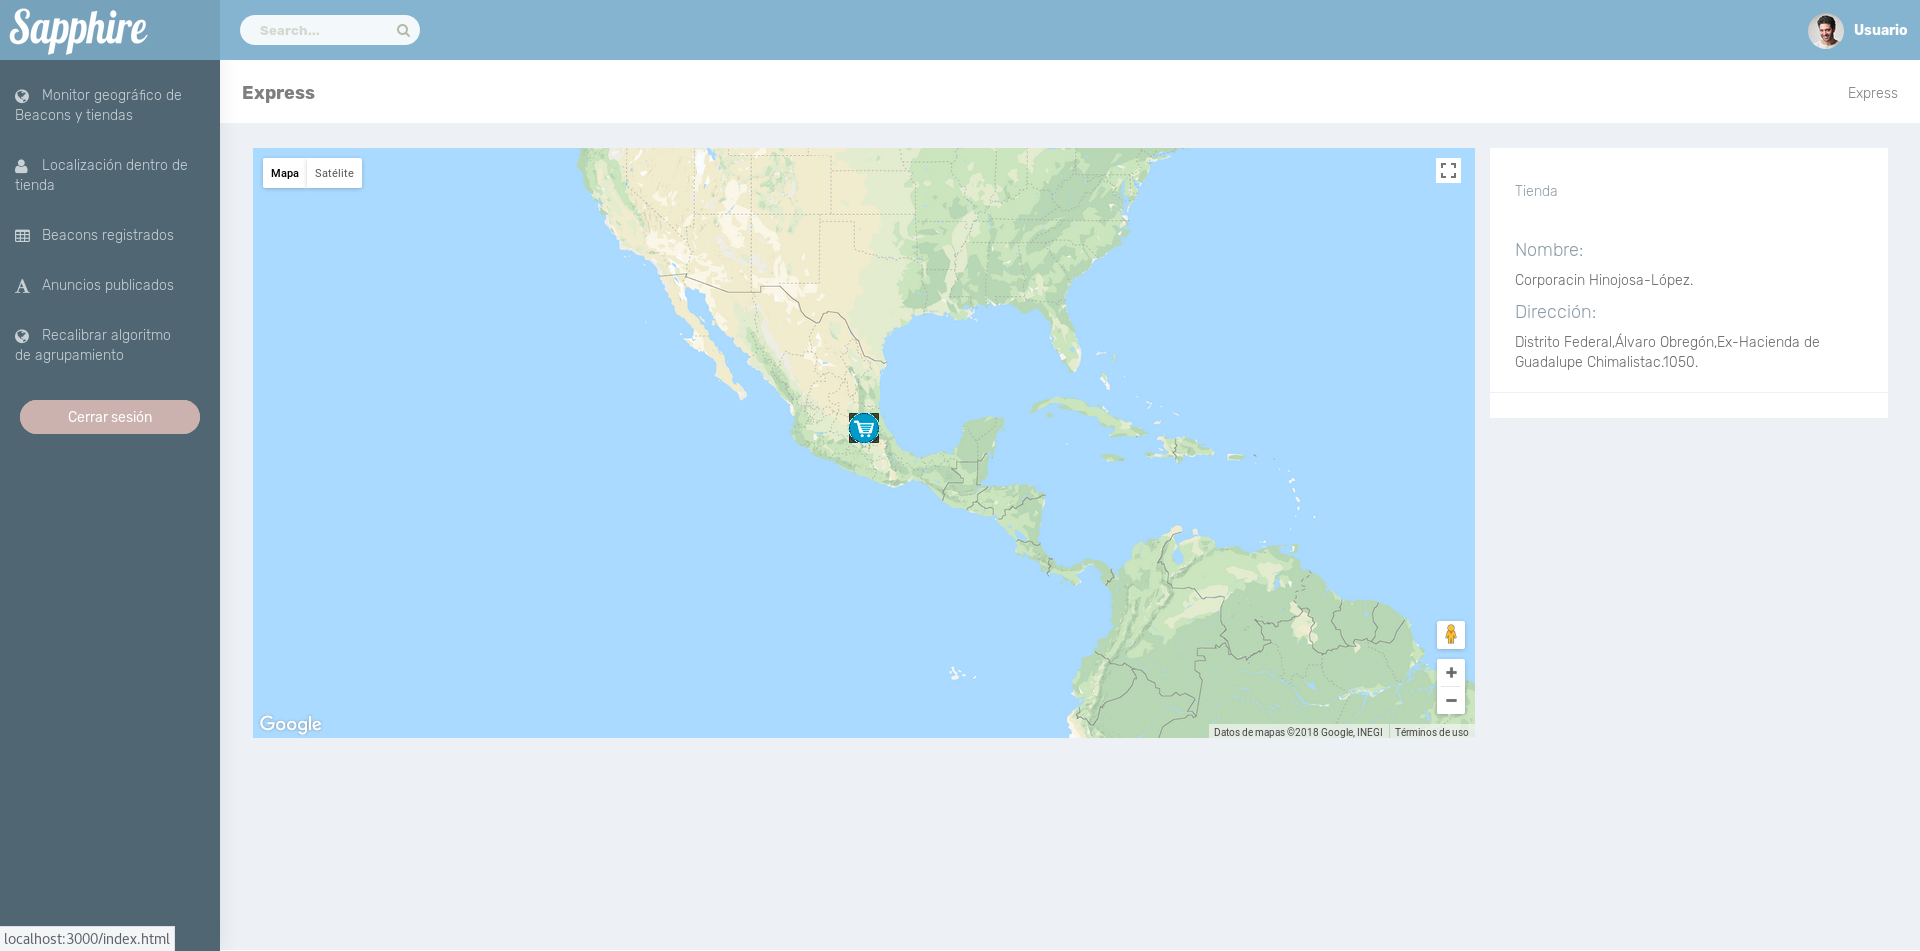
\includegraphics[width=.9 \textwidth]{imagenes/panelAdmin/monitorComputadora}
		\caption{UIPanel3: Monitor Beacons y tiendas computadora.}
		\label{PA:3}
\end{figure}
\FloatBarrier

La Figura \ref{PA:4} muestra como se ve la interfaz de usuario del Panel de Administración para el monitor de Beacons y tiendas desde una tableta.
\FloatBarrier
\begin{figure}[htbp!]
		\centering
			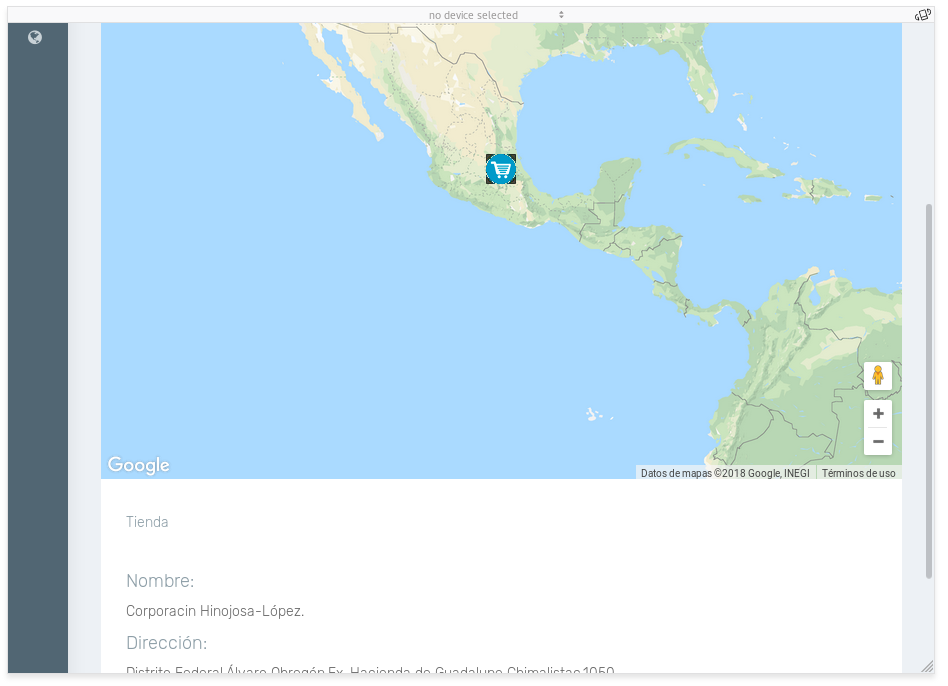
\includegraphics[width=.9 \textwidth]{imagenes/panelAdmin/tabmonitor}
		\caption{UIPanel4: Monitor Beacons y tiendas tableta.}
		\label{PA:4}
\end{figure}
\FloatBarrier



La figura \ref{PA:flujo4} muestra como es el flujo de navegación general del Panel de Admnistración.

\FloatBarrier
\begin{figure}[htbp!]
		\centering
			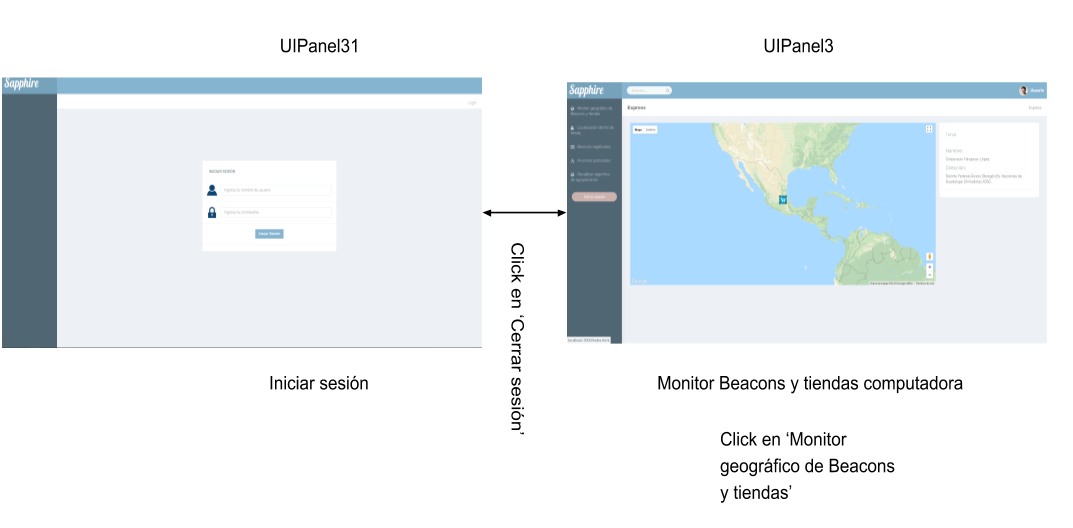
\includegraphics[width=1 \textwidth]{imagenes/paneladminmapa/general2}
		\caption{Flujo de navegación general Panel de Administración.}
		\label{PA:flujo4}
\end{figure}
\FloatBarrier